\chapter{Kalman Filters}

Il presente capitolo illustra alcuni esperimenti condotti sui Kalman filters e analizza i risultati ottenuti.

\section{Implementazione e librerie di supporto}
Come consigliato si è fatto uso della libreria Java EJML, la quale mette a disposizione una comoda rappresentazione delle matrici e delle relative operazioni. In particolar modo si è sfruttata la classe \texttt{SimpleMatrix} che permette di esprimere le operazioni tra matrici in modo astratto, facilitando di molto la lettura del codice a scapito di un'efficienza leggermente minore. È stata quindi implementata la classe \texttt{KalmanFilter}, utilizzata per eseguire tutti i test di seguito riportati.

\section{Simulazione di un processo}

Il processo scelto è lo spostamento un oggetto che si muove di moto uniformemente accelerato in due dimensioni (piano XY). Lo stato è quindi rappresentato dal vettore:
\begin{equation*}
\textbf{x} = 
\begin{bmatrix}
x \\
y \\
v_x \\
v_y \\
\end{bmatrix}
\qquad
\end{equation*}

dove le componenti $x$ e $y$ rappresentano la posizione corrente dell'oggetto, mentre $v_x$ e $v_y$ rappresentano la velocità dello stesso.

La matrice di transizione di stato \textbf{A}, la matrice di control input \textbf{B} e il relativo vettore di control input \textbf{u} sono così definiti:

\begin{equation*}
\textbf{A} = 
\begin{bmatrix}
1 & 0 & \dt & 0 \\
0 & 1 & 0 & \dt \\
0 & 0 & 1 & 0 \\
0 & 0 & 0 & 1 \\
\end{bmatrix}
\qquad 
\textbf{B} = 
\begin{bmatrix}
\frac{1}{2}\dt^2 & 0\\
0 & \frac{1}{2}\dt^2\\
\dt & 0 \\
0 & \dt \\
\end{bmatrix}
\qquad 
\textbf{u} = 
\begin{bmatrix}
a_x \\
a_y \\
\end{bmatrix}
\end{equation*}
dove $\dt$ indica l'intervallo di tempo trascorso, idealmente, tra un'iterazione e la successiva (espresso in secondi). Poiché il modello di transizione di stato prevede che il prossimo stato (predetto) $\textbf{x}^{(p)}_{t+1}$ sia calcolato come $\textbf{x}^{(p)}_{t+1} = \textbf{Ax}+ \textbf{Bu}$, le entry delle  matrici sono tali da implementare le note leggi del moto uniformemente accelerato di seguito riportate:
\begin{equation*}
s' = s + v \dt + \frac{1}{2}a(\dt)^2  \qquad v' = v + a \dt
\end{equation*}
In particolare il vettore \textbf{u}, se assunto costante, permette di mantenere l'accelerazione invariata; tale assunzione può essere facilmente rilassata per modellare anche quei casi in cui l'accelerazione subisce delle variazioni note. In tutti i test condotti \textbf{u} è assunto costante ma l'accelerazione subisce comunque delle variazioni dovute al rumore di processo: essa è infatti soggetta a rumore che segue le distribuzioni gaussiane $\mathcal{N}(0; \sigma^2_{accX})$ e $\mathcal{N}(0; \sigma^2_{accY})$, rispettivamente per la componente x e y. Vista la particolare influenza che i cambiamenti di accelerazione hanno su posizione e velocità dell'oggetto, la matrice di covarianza del rumore di processo \textbf{Q} è definita come:
\begin{equation*}
\textbf{Q} = 
\begin{bmatrix}
(\frac{1}{2} \dt^2 \sigma_{accX})^2 & 0 & 0 & 0 \\
0 & (\frac{1}{2} \dt^2 \sigma_{accY})^2 & 0 & 0 \\
0 & 0 & (\dt \sigma_{accX})^2 & 0 \\
0 & 0 & 0 & (\dt \sigma_{accY})^2 \\
\end{bmatrix}
\end{equation*}
per semplicità si è utilizzata una matrice diagonale, assumendo che tutte le variabili di stato osservate siano tra loro indipendenti. Questo ovviamente non rispecchia fedelmente la realtà: posizione e velocità sono inevitabilmente legate tra di loro in quanto influenzate dalle stesse variazioni di accelerazione.

Le misurazioni si limitano invece alla sola posizione dell'oggetto: si simula pertanto una situazione in cui nessuna informazione relativa alla velocità viene resa disponibile al Kalman filter per mezzo di ipotetici sensori. 
Anche le misura di posizione è soggetta a rumore, che in questo caso segue le distribuzioni gaussiane $\mathcal{N}(0,\sigma^2_{posX})$ e $\mathcal{N}(0,\sigma^2_{posY})$; la relativa matrice di covarianza è definita di conseguenza come:
\begin{equation*}
\textbf{R} = 
\begin{bmatrix}
\sigma^2_{posX} & 0 \\
0 & \sigma^2_{posY} \\
\end{bmatrix}
\end{equation*}
Anche in questo caso si è utilizzata per semplicità una matrice diagonale, assumendo che le misurazioni dei sensori di posizione (e relativi errori) siano tra loro indipendenti.

È quindi possibile intervenire separatamente sulle deviazioni standard $\sigma_{accX}, \sigma_{accY}, \sigma_{posX}$ e $\sigma_{posY}$ per incrementare/diminuire a piacere il rumore cui sono soggetti il processo reale e le misurazioni ottenute dai sensori.

\subsection{Prestazioni al variare dell'errore}

Sono stati effettuati alcuni test variando sia il rumore di processo che quello di misurazione al fine di valutare le prestazioni del Kalman filter in diverse condizioni. Per semplicità in tutti i casi si è assunto $\sigma_{accX} = \sigma_{accY}$ e $\sigma_{posX} = \sigma_{posY}$;
nelle considerazioni che seguono si farà pertanto riferimento alle sole $\sigma_{acc}$ e $\sigma_{pos}$. Inoltre, lo stato iniziale reale e stimato non coincidono: si è infatti posto lo stato iniziale stimato $\mathbf{x_0} = \begin{bmatrix} 0 & 0 & 0 & 0 \end{bmatrix}^T$ e la relativa matrice di covarianza $\mathbf{P_0 = I}$, mentre lo stato reale è stato inizializzato come $\mathbf{x_{real}} = \begin{bmatrix} 5 & 20 & 3 & -3 \end{bmatrix}^T$. Infine, si è posto $\dt = 1$.

Se non diversamente specificato, in tutti grafici che seguono (per esigenze di rappresentazione) vengono riportati solo i dati relativi alla componente $x$ della posizione: valore reale, valore stimato e valore osservato.

\begin{itemize}
\item \textbf{Errore trascurabile}\\
In questo primo caso sono state poste $\sigma_{acc} = 0$ e $\sigma_{pos} = 10^{-5}$ per simulare una condizione in cui il processo reale segue fedelmente il modello e la misurazione dei sensori è pressoché perfetta. Si ricordi tuttavia che lo stato iniziale del Kalman filter e quello del processo reale non coincidono in questo primo scenario. Non è stato possibile predisporre un errore di misurazione nullo: infatti \textbf{P} tende rapidamente ad annullarsi e, se si assume anche \textbf{R} nulla, dopo poche iterazioni l'inversione della matrice $\mathbf{S = H P H^T + R}$  (operazione necessaria per il calcolo del Kalman Gain) fallisce in quanto la matrice risultante ha determinante nullo. 

Ad ogni modo, ponendosi nelle condizioni di errore trascurabile presentante inizialmente, dopo sole 4 iterazioni lo scarto tra variabili di stato reali e stimate risulta in media inferiore di $10^{-5}$. Inoltre la matrice \textbf{P} assume il seguente aspetto:
\begin{equation*}
\textbf{P} = 
\begin{bmatrix}
7 \times 10^{-9} & 0 & 3 \times 10^{-9} & 0 \\
0 & 7 \times 10^{-9} & 0 & 3 \times 10^{-9} \\
3 \times 10^{-9} & 0 & 2 \times 10^{-9} & 0 \\
0 & 3 \times 10^{-9} & 0 & 2 \times 10^{-9} \\
\end{bmatrix}
\end{equation*}
ovvero l'errore commesso nell'approssimare lo stato reale è praticamente nullo, come previsto. Si noti come emerge ugualmente una correlazione fra posizione e velocità per le componenti analoghe.

\item\textbf{Errore basso}\\
Per modellare una situazione più realistica si sono poste $\sigma_{acc} = 3$ e $\sigma_{pos} = 6$. In queste condizioni il Kalman filter approssima molto bene il processo, e recupera in fretta lo ``scarto" dovuto alle diverse condizioni iniziali.

\begin{minipage}{\linewidth}
	\centering
	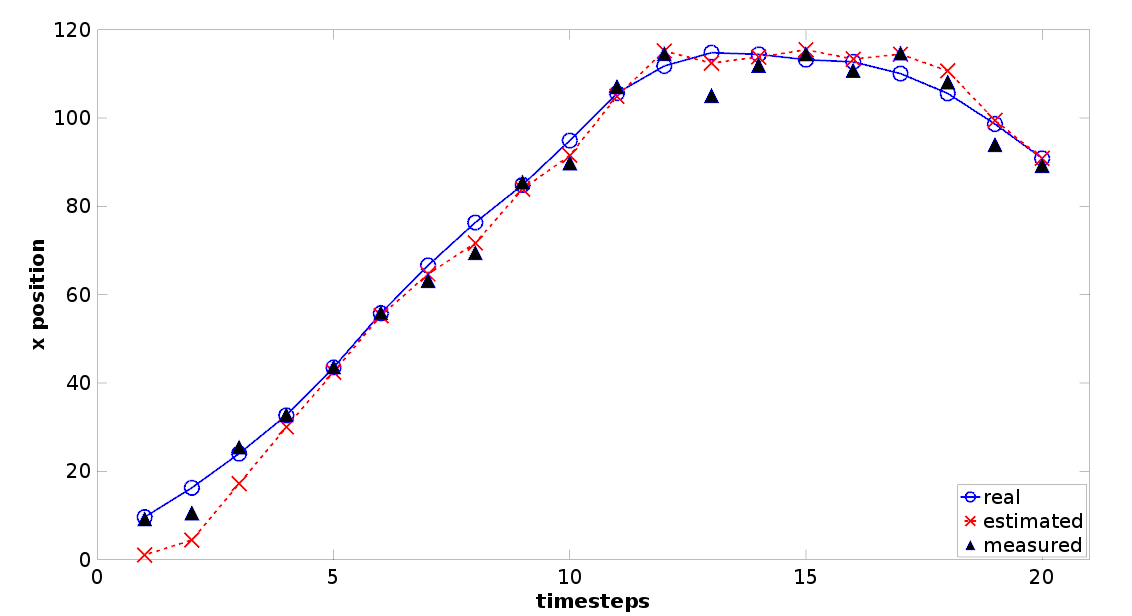
\includegraphics[width=\linewidth]{a3m6}
	\captionof{figure}{Stima nelle prime 20 iterazioni ponendo $\sigma_{acc} = 3$ e $\sigma_{pos} = 6$.}  
\end{minipage}

\item\textbf{Errore medio}\\
Si sono poste $\sigma_{acc} = 15$ e $\sigma_{pos} = 30$. In questo caso il rumore sembra influenzare maggiormente le prestazioni dello stimatore, come si evince dai due casi di seguito riportati. Il primo caso è da considerarsi ``fortunato" in quanto le misurazioni dei sensori seguono abbastanza fedelmente il processo reale; ciò consente al Kalman filter di fornire un'approssimazione tutto sommato buona. Nel secondo caso, invece, i valori osservati sono soggetti a delle oscillazioni più significative: queste hanno ripercussioni negative sulla stima.

\begin{minipage}{\linewidth}
	\centering
	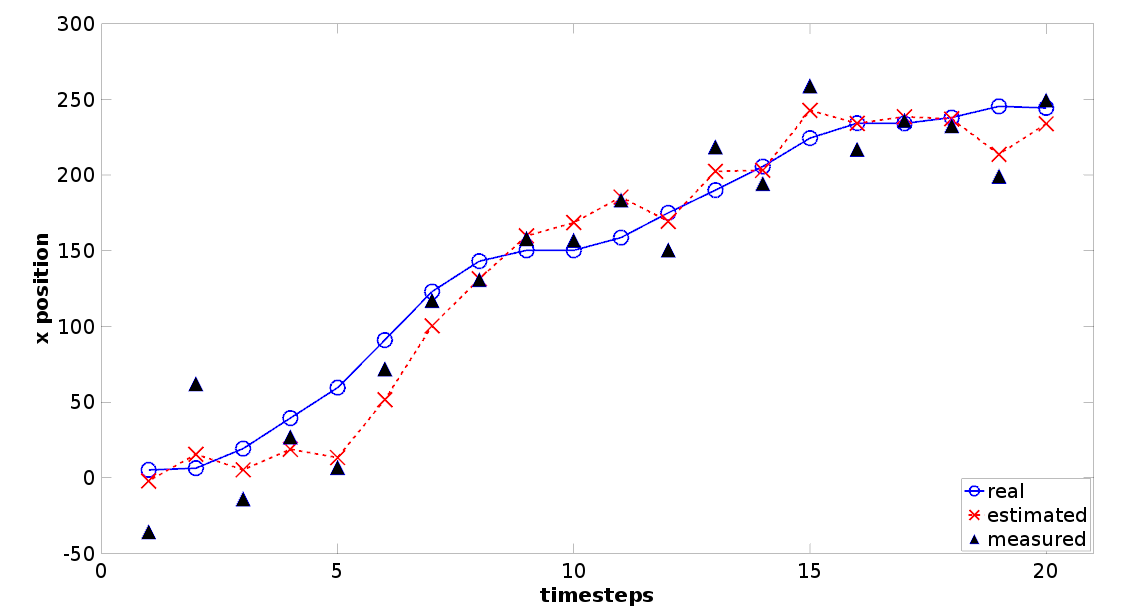
\includegraphics[width=\linewidth]{a15m30}
	\captionof{figure}{Stima nelle prime 20 iterazioni ponendo $\sigma_{acc} = 15$ e $\sigma_{pos} = 30$. Un caso ``fortunato" in cui le misurazioni non si discostano troppo dai valori reali.}  
\end{minipage}

\begin{minipage}{\linewidth}
	\centering
	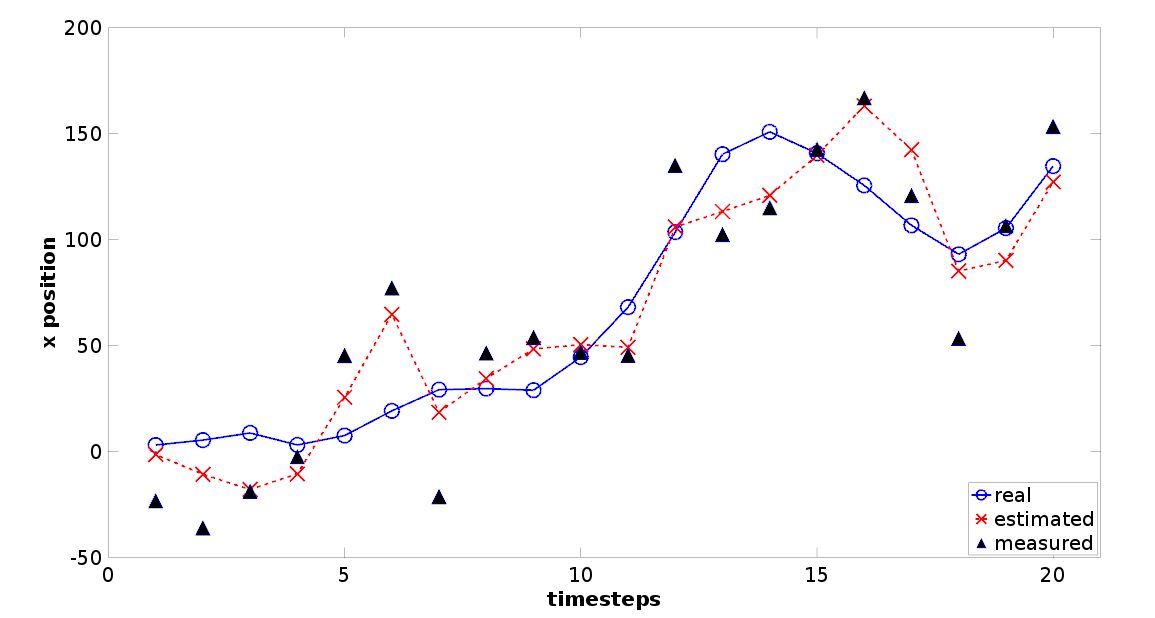
\includegraphics[width=\linewidth]{a15m30_2}	
	\captionof{figure}{Stima nelle prime 20 iterazioni ponendo $\sigma_{acc} = 15$ e $\sigma_{pos} = 30$. Un caso meno fortunato.}  
\end{minipage}

%\begin{center}
%\setlength\extrarowheight{2pt} % for a bit of visual "breathing space"
%\begin{tabularx}{0.8\textwidth}{|C|C|C|}
%\hline
%\textbf{Tolleranza componenti posizione} & \textbf{Tolleranza componenti velocità} & \textbf{Percentuale iterazioni entro le tolleranze}  \\\hline
%4 m & 4 m/s & $\sim$31\%\\
%\hline
%5 m & 5 m/s & $\sim$52\%\\
%\hline
%6 m & 6 m/s & $\sim$75\%\\
%\hline
%7 m & 7 m/s & $\sim$82\%\\
%\hline
%\end{tabularx}
%\end{center}

\newpage

\item\textbf{Errore elevato}\\
Infine, è stata trattata una situazione estrema ponendo $\sigma_{acc} = 50$ e $\sigma_{pos} = 100$. Si riportano di nuovo due diversi casi: in entrambi è possibile osservare come il Kalman filter non riesca a fornire consistentemente delle stime accurate a causa dell'elevata incertezza sia sul processo che sulle osservazioni. Durante alcune iterazioni il valore di posizione stimato e quello reale differiscono di quasi 200 metri, rendendo il tracking dell'oggetto molto difficoltoso.

\begin{minipage}{\linewidth}
	\centering
	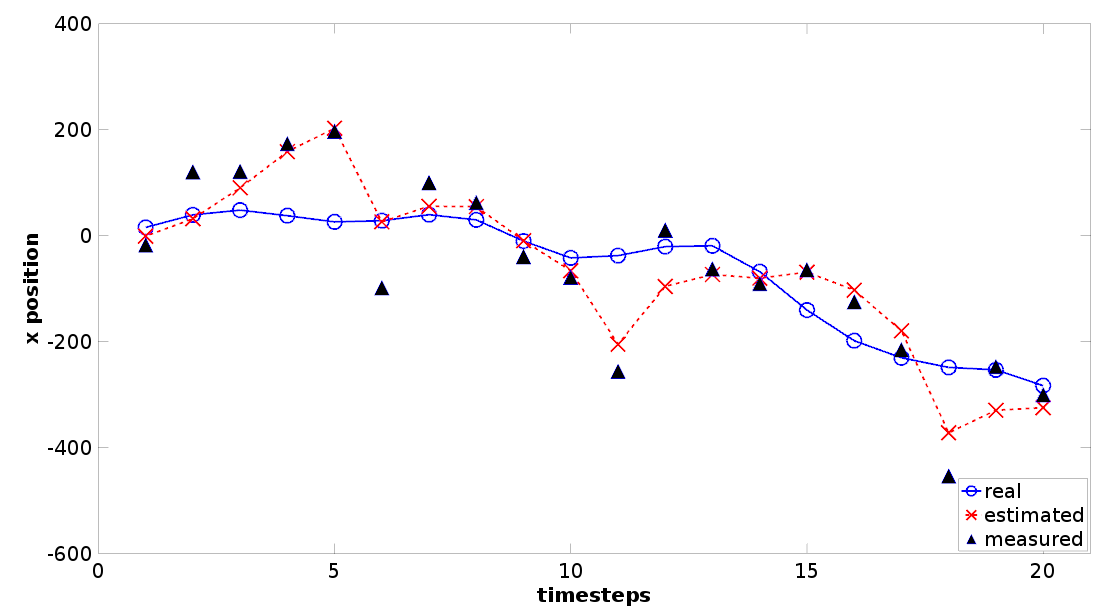
\includegraphics[width=\linewidth]{a50m100}
	\captionof{figure}{Stima nelle prime 20 iterazioni ponendo $\sigma_{acc} = 50$ e $\sigma_{pos} = 100$. Un primo caso.}  
\end{minipage}

\begin{minipage}{\linewidth}
	\centering
	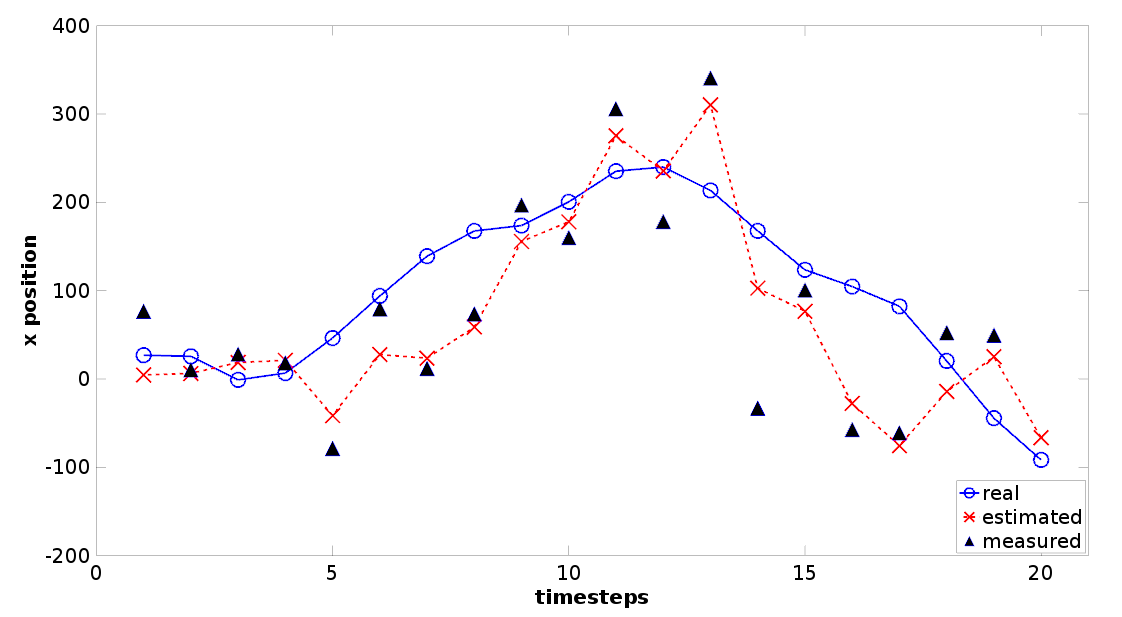
\includegraphics[width=\linewidth]{a50m100_2}
	\captionof{figure}{Stima nelle prime 20 iterazioni ponendo $\sigma_{acc} = 50$ e $\sigma_{pos} = 100$. Un secondo caso.}  
\end{minipage}

\newpage

\item \textbf{Errore di processo elevato ed errore di misurazione nullo}\\
Nel primo dei due casi si è posto $\sigma_{acc} = 100$ e $\sigma_{pos} = 0$. La matrice \textbf{P} si stabilizza già dopo le prime iterazioni, assumendo la forma:
\begin{equation*}
\small
\textbf{P} = 
\begin{bmatrix}
0 & 0 & 0 & 0 \\
0 & 0 & 0 & 0 \\
0 & 0 & 12071 & 0 \\
0 & 0 & 0 & 12071 \\
\end{bmatrix}
\end{equation*}
Tale risultato può essere intuitivamente giustificato come segue: poiché si ha la certezza che le misurazioni sono sempre perfettamente accurate, la varianza delle variabili di stato che rappresentano la posizione dell'oggetto è nulla; al contrario, poiché l'accelerazione è soggetta ad un rumore significativo, la varianza della velocità (e quindi l'incertezza sul suo valore reale) assume valori estremamente elevati. In figura \ref{velocity} sono riportati i dati relativi alla stima della velocità (componente x) in due differenti casi, che come previsto è piuttosto inaccurata a causa del rumore di processo.

\begin{minipage}{\linewidth}
	\centering
	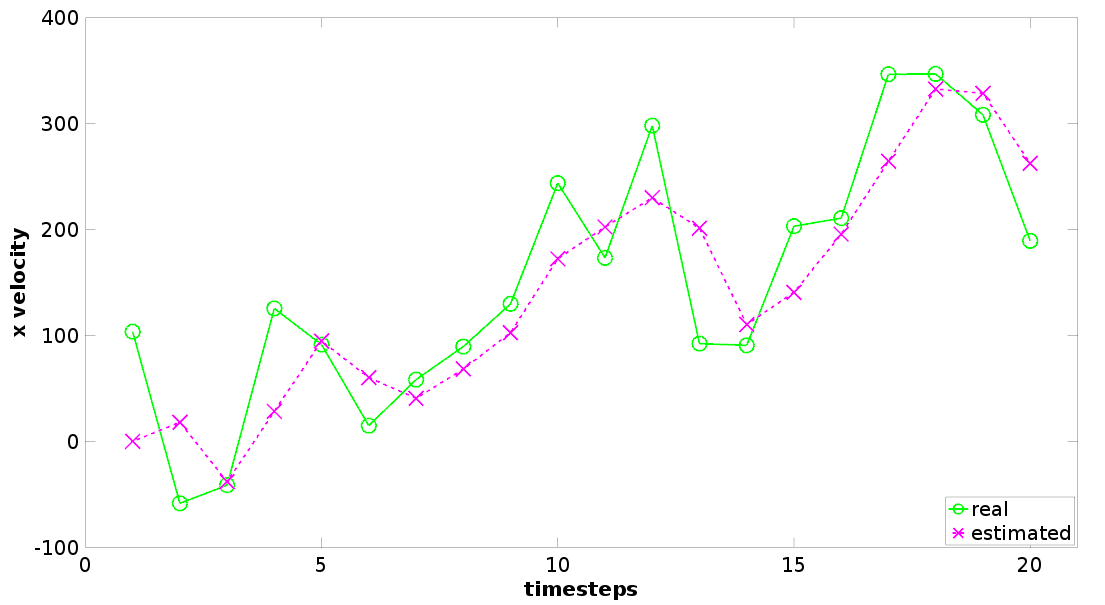
\includegraphics[width=\linewidth]{velocity}
	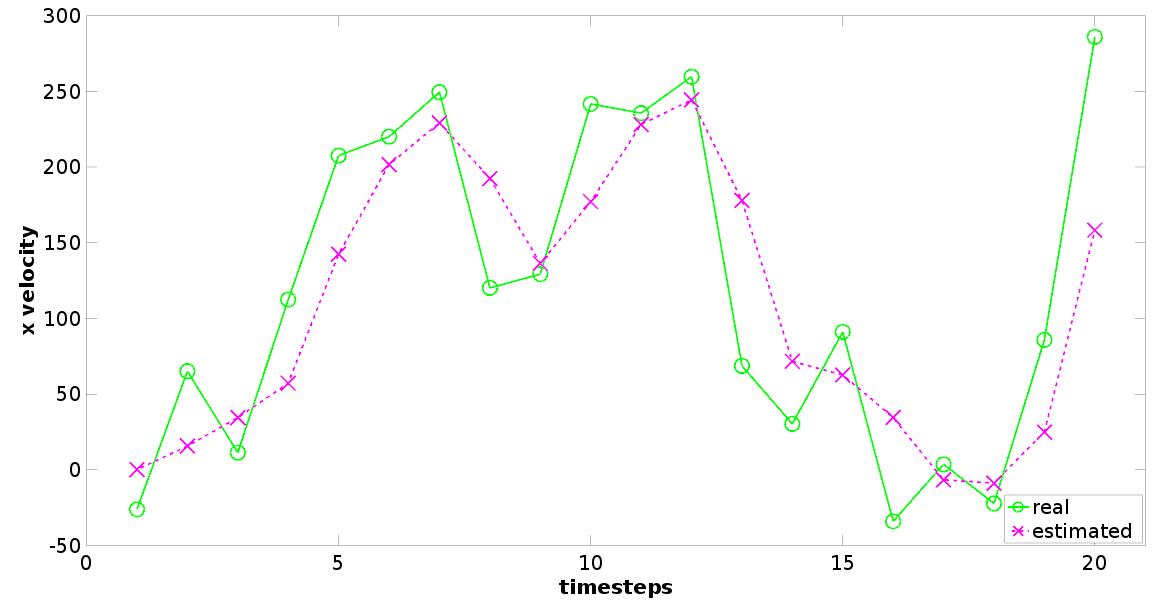
\includegraphics[width=\linewidth]{velocity2}
	\captionof{figure}{Stima nelle prime 20 iterazioni ponendo $\sigma_{acc} = 50$ e $\sigma_{pos} = 100$.}  
	\label{velocity}
\end{minipage}

\newpage

\item \textbf{Errore di processo nullo ed errore di misurazione elevato}\\
Simmetricamente, il secondo caso prevede $\sigma_{acc} = 0$ e $\sigma_{pos} = 100$. Le prime 20 iterazioni mostrano un andamento piuttosto stabile, come si evince dalla figura \ref{a0m100}.

\begin{minipage}{\linewidth}
	\centering
	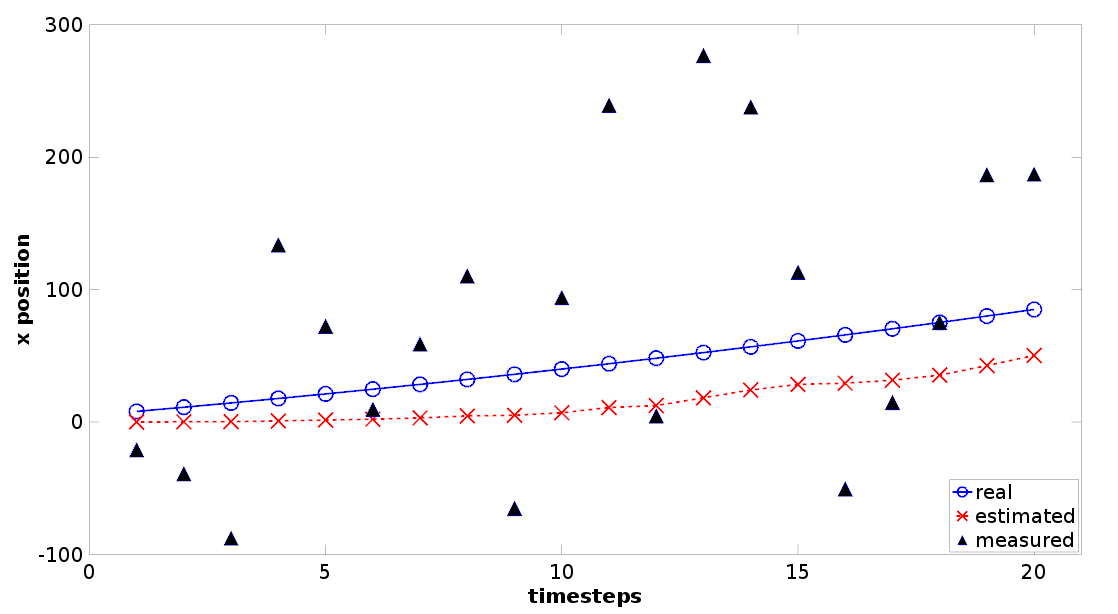
\includegraphics[width=\linewidth]{a0m100}
	\captionof{figure}{Stima nelle prime 20 iterazioni ponendo $\sigma_{acc} = 0$ e $\sigma_{pos} = 100$.}  
	\label{a0m100}
\end{minipage}

Pertanto, si è deciso di effettuare un numero maggiore di iterazioni per indagare il comportamento del Kalman filter sul lungo periodo. Dopo rispettivamente 500, 2500 e 5000 iterazioni la matrice \textbf{P} assume le seguenti forme: 

\begin{equation*}
\small
\textbf{P}_{500}= 
\begin{bmatrix}
60 & 0 & 1.2 & 0 \\
0 & 60 & 0 & 1.2 \\
1.2 & 0 & 0.0002 & 0 \\
0 & 1.2 & 0 &  0.0002 \\
\end{bmatrix}
\;
\textbf{P}_{2500} = 
\begin{bmatrix}
12.2 & 0 & 0.005 & 0 \\
0 & 12.2 & 0 & 0.005 \\
0.005 & 0 & 2.2 \times 10^{-6} & 0 \\
0 & 0.005 & 0 &  2.2\times 10^{-6} \\
\end{bmatrix}
\end{equation*}
\begin{equation*}
\small
\textbf{P}_{5000} = 
\begin{bmatrix}
6.2 & 0 & 0.001 & 0 \\
0 & 6.2 & 0 & 0.001 \\
0.001 & 0 & 3.2\times 10^{-7} & 0 \\
0 & 0.001 & 0 &  3.2\times 10^{-7} \\
\end{bmatrix}
\end{equation*}

La giustificazione di questo risultato è meno intuitiva. La spiegazione che è sembrata più verosimile è la seguente: si sa per certo che il processo viene simulato alla perfezione; infatti, il fenomeno reale non è affetto da alcun tipo di rumore e pertanto si comporta esattamente come previsto dal modello. Tuttavia, il Kalman filter non ha informazioni riguardo allo stato iniziale del processo reale, né può ricavarlo con assoluta sicurezza dalle misurazioni in quanto molto rumorose: per questo motivo vi è sempre un minimo di incertezza nella stima dello stato corrente (che tende a diminuire con l'aumentare delle misurazioni effettuate). Tale incertezza riguarda solo la posizione (poiché non si  hanno certezze riguardo al punto di partenza) e non la velocità, che viene stimata praticamente senza errori grazie al modello.
\end{itemize}

\subsection{Prestazioni al variare delle condizioni iniziali}
\label{known_state_subsec}

Alcuni dei test presentati nella sezione precedente sono stati ripetuti variando le condizioni iniziali, al fine di comprendere come queste influenzino la stima durante le iterazioni successive. Sono stati predisposti due scenari; in entrambi i casi il Kalman filter parte dallo stato iniziale $\mathbf{x_0} = \begin{bmatrix} 0 & 0 & 0 & 0 \end{bmatrix}^T$. Nel primo caso il processo reale parte dal medesimo stato (partenza perfetta), mentre nel secondo si impone arbitrariamente $\mathbf{x_{real}} = \begin{bmatrix} 220 & -137 & 17 & 28 \end{bmatrix}^T$ (partenza falsata). In caso di partenza perfetta si è posta $\mathbf{P_0 = 0}$ così che l'incertezza sullo stato stimato iniziale sia nulla.

\begin{itemize}
\item \textbf{Errore basso}\\
Sono state riprese le condizioni del primo test della sezione precedente, ponendo $\sigma_{acc} = 3$ e $\sigma_{pos} = 6$.
I risultati sono riassunti dai grafici nella figura \ref{ws_a3m6}. È possibile notare come nel caso con partenza perfetta il Kalman filter approssimi decisamente bene il processo, facilitato anche dal basso rumore. Nel caso con partenza falsata, invece, il divario tra posizione stimata e reale viene colmato in poche iterazioni.

\begin{minipage}{\linewidth}
	\centering
	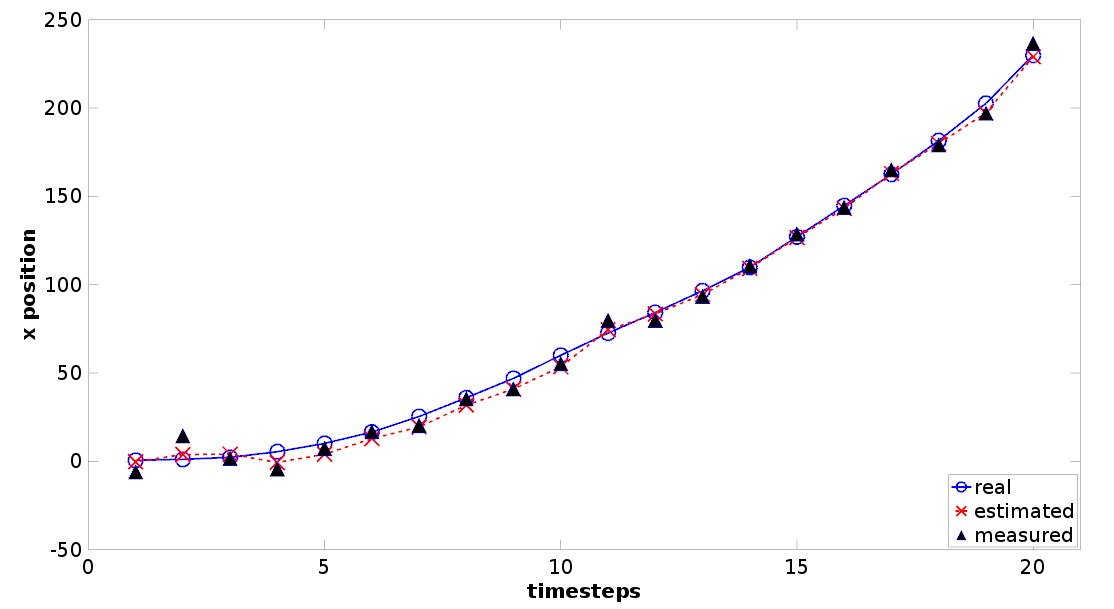
\includegraphics[width=0.9\linewidth]{ps_a3m6}
	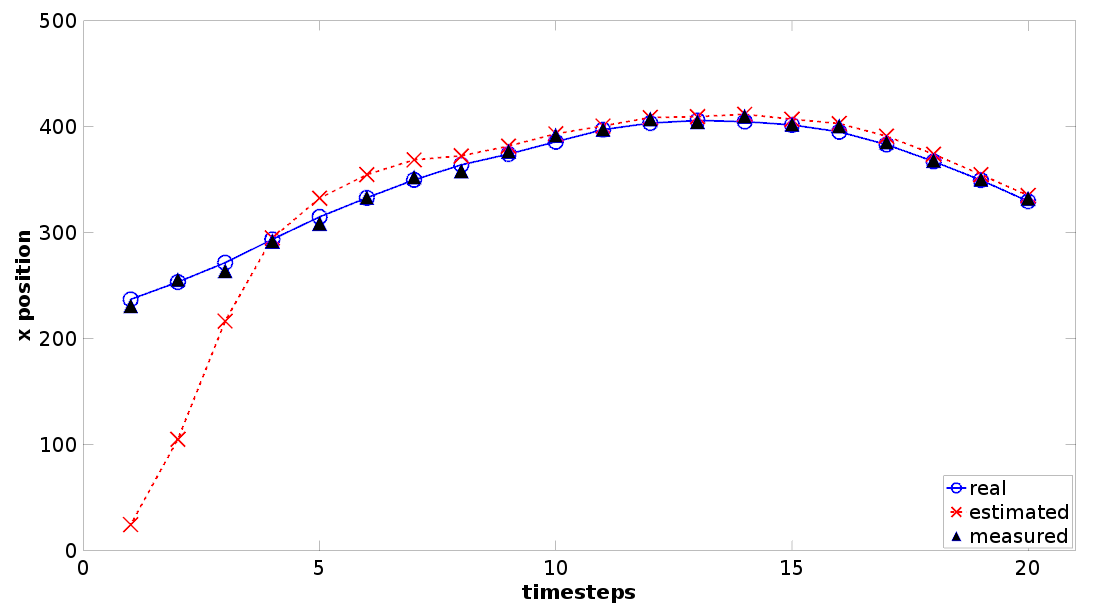
\includegraphics[width=0.9\linewidth]{ws_a3m6}
	\captionof{figure}{Stima nelle prime 20 iterazioni ponendo $\sigma_{acc} = 3$ e $\sigma_{pos} = 6$ (rispettivamente con partenza perfetta e falsata).} 
	\label{ws_a3m6} 
\end{minipage}

\item \textbf{Errore elevato}\\
Ponendo $\sigma_{acc} = 50$ e $\sigma_{pos} = 100$, anche una partenza perfetta non è sufficiente per mantenere l'approssimazione vicina al processo reale: dopo le prime iterazioni il Kalman filter viene deviato dalle osservazioni estremamente rumorose (figura \ref{ps_a50m100}). Sorprendentemente, lo stimatore è comunque in grado di approssimare (perlomeno a grandi linee) l'andamento generale del processo reale anche in queste situazioni estreme; ciò è vero soprattutto quando una serie di misurazioni si rivelano piuttosto precise, come accade nel caso illustrato in figura \ref{ws_a50m100} (decima iterazione e successive).

\begin{minipage}{\linewidth}
	\centering
	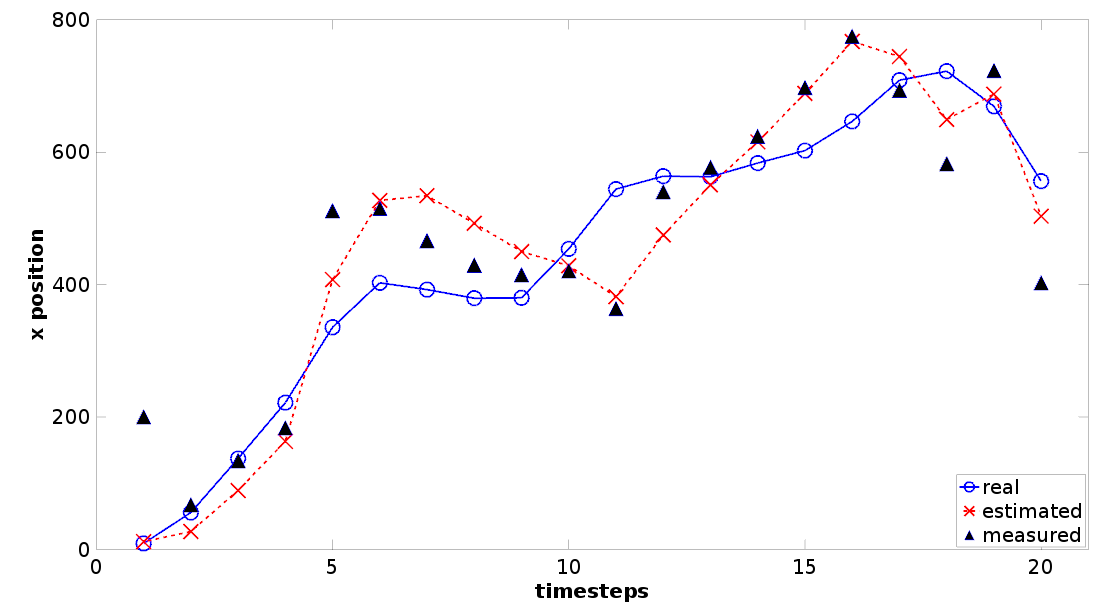
\includegraphics[width=\linewidth]{ps_a50m100}
	\captionof{figure}{Stima nelle prime 20 iterazioni ponendo $\sigma_{acc} = 50$ e $\sigma_{pos} = 100$ (partenza perfetta).}  
	\label{ps_a50m100}
\end{minipage}

\begin{minipage}{\linewidth}
	\centering
	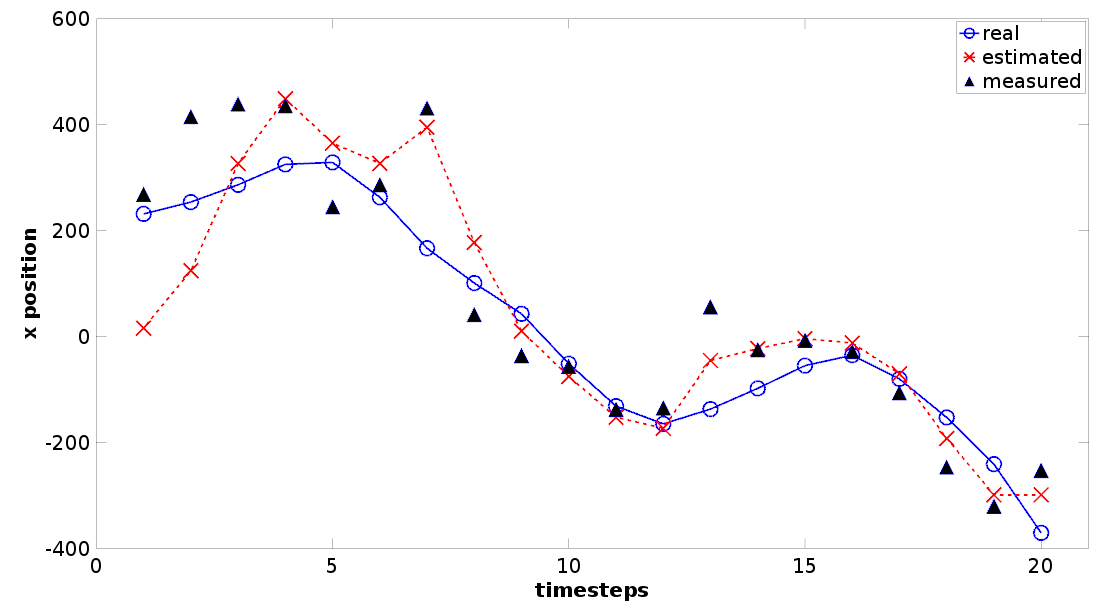
\includegraphics[width=\linewidth]{ws_a50m100}
	\captionof{figure}{Stima nelle prime 20 iterazioni ponendo $\sigma_{acc} = 50$ e $\sigma_{pos} = 100$ (partenza falsata).}  
	\label{ws_a50m100}
\end{minipage}

\newpage

\item \textbf{Errore di processo nullo ed errore di misurazione elevato}\\
In precedenza si è osservato come, nel caso in cui si pongano  $\sigma_{acc} = 0$ e $\sigma_{pos} = 100$, lo stimatore tenda a favorire il modello nella predizione dello stato successivo, in quanto esente da rumore. Questo fa sì che lo stato iniziale ricopra un ruolo importante: con una partenza perfetta il Kalman filter è in grado di simulare esattamente il processo reale, come testimonia la figura \ref{ps_a0m100}. Anche nel caso in cui lo stato iniziale stimato e quello reale non coincidano l'errore tende lentamente a diminuire con il passare delle iterazioni (figura \ref{ws_a0m100_long}): per quanto falsata possa essere la partenza, sul lungo periodo l'aumentare del numero di evidenze disponibili fa sì che il Kalman filter alteri la propria traiettoria, allineandosi progressivamente al processo reale.

\begin{minipage}{\linewidth}
	\centering
	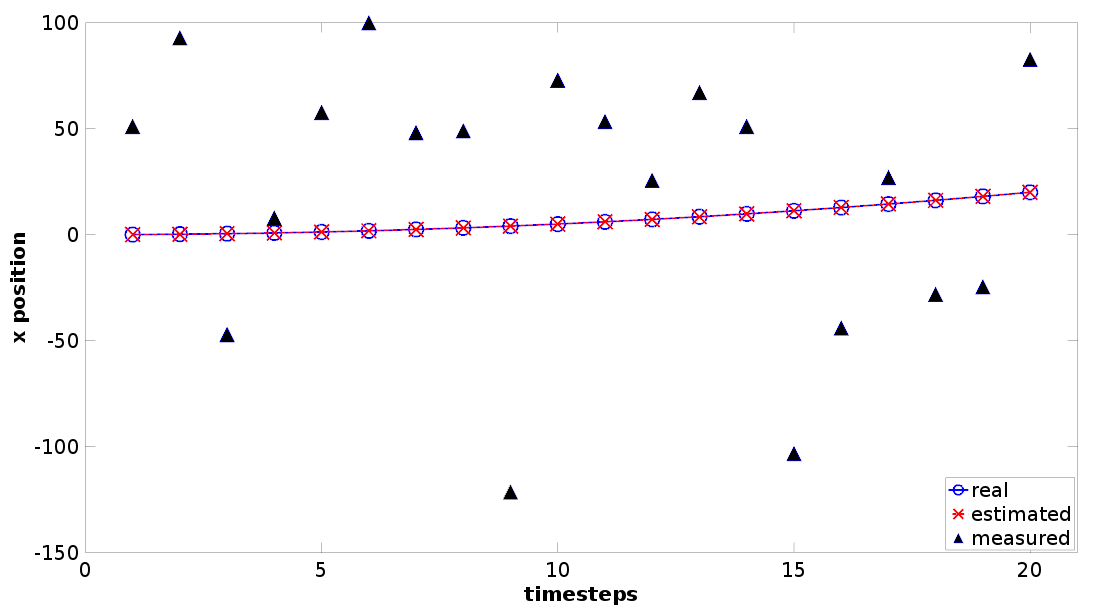
\includegraphics[width=\linewidth]{ps_a0m100}
	\captionof{figure}{Stima nelle prime 20 iterazioni ponendo $\sigma_{acc} = 0$ e $\sigma_{pos} = 100$ (partenza perfetta).} 
	\label{ps_a0m100} 
\end{minipage}

\begin{minipage}{\linewidth}
	\centering
	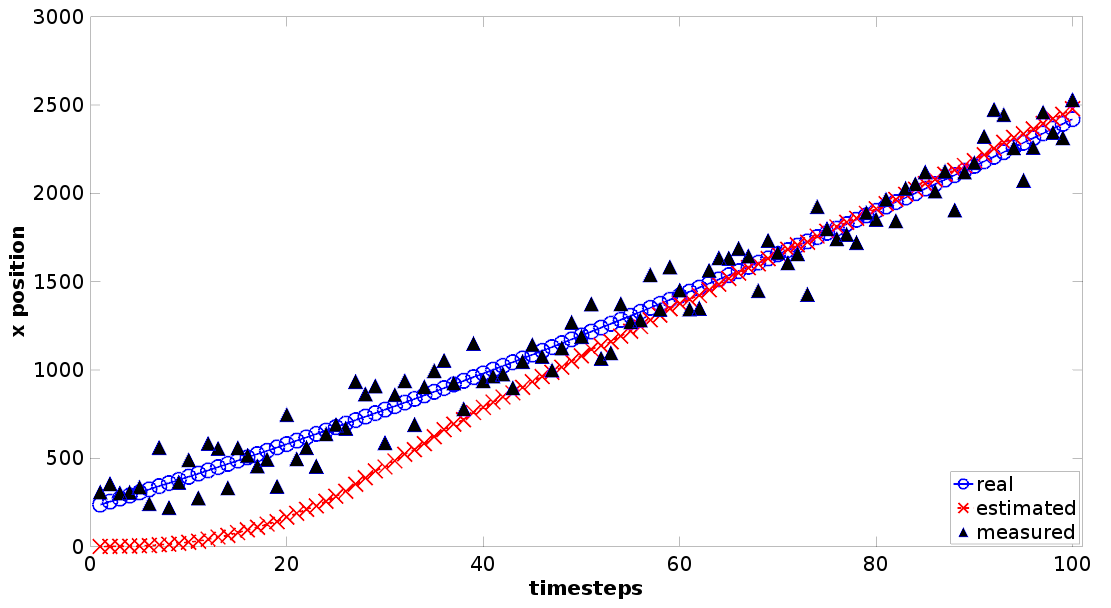
\includegraphics[width=\linewidth]{ws_a0m100_long}
	\captionof{figure}{Stima nelle prime 100 iterazioni ponendo $\sigma_{acc} = 0$ e $\sigma_{pos} = 100$ (partenza falsata).} 
	\label{ws_a0m100_long}
\end{minipage}

\end{itemize}

\section{Simulazione di un processo non lineare}

Il Kalman filter è interamente specificato tramite matrici; pertanto, esso si presta a modellare unicamente quei processi che presentano transizioni di stato lineari. Si può dimostrare che se la distribuzione di probabilità è una gaussiana multivariata e il modello di transizione è lineare, applicare l'operazione di filtering in un modello probabilistico temporale ha come risultato un'altra distribuzione gaussiana multivariata. Il modello di transizione lineare è quindi un'assunzione necessaria per garantire la convergenza del metodo. Per questo motivo il Kalman filter non è adatto a simulare processi non lineari, come dimostra il seguente esperimento.

Il processo che si vorrebbe simulare è l'evoluzione della coppia $\langle x, x^2 \rangle$ al variare di $x$. Nel caso in esame si assume che $x$ venga incrementata di una quantità costante $\dx > 0$ ad ogni iterazione. Pertanto, fissato $\dx$, idealmente lo stato corrente \textbf{x} e quello successivo \textbf{x'} sono rappresentati dai vettori:
\begin{equation*}
\textbf{x} = 
\begin{bmatrix}
x^2 \\
x \\
\end{bmatrix}
\qquad
\textbf{x'} = 
\begin{bmatrix}
(x + \dx)^2 \\
x + \dx \\
\end{bmatrix}
\end{equation*}
Poiché la transizione di stato deve essere espressa linearmente si è fatto ricorso alla formula di Taylor di ordine 1, applicata alla funzione $x^2$ (ponendo $a = 1$):
\begin{equation}
\label{eq_taylor}
f(x) \approx f(a) + f'(a)(x-a) \qquad \mapsto  \qquad x^2 \approx 1 + 2(x-1)
\end{equation}
La matrice di transizione di stato \textbf{A}, la matrice di control input \textbf{B} e il relativo vettore di control input \textbf{u} sono definiti di conseguenza come :
\begin{equation*}
\textbf{A} = 
\begin{bmatrix}
0 & 2 \\
0 & 1 \\
\end{bmatrix}
\qquad 
\textbf{B} = 
\begin{bmatrix}
1 & 0\\
0 & 1\\
\end{bmatrix}
\qquad 
\textbf{u} = 
\begin{bmatrix}
2\dx -1 \\
\dx \\
\end{bmatrix}
\end{equation*}
In questo modo, lo stato successivo predetto dal modello è:
\begin{equation*}
\mathbf{x}^{(p)}_{t+1} = \mathbf{A x + B u} = 
\begin{bmatrix}
2x + 2\dx -1 \\
x + \dx \\
\end{bmatrix}  = 
\begin{bmatrix}
1 + 2(x + \dx -1) \\
x + \dx \\
\end{bmatrix} 
\end{equation*}
in accordo con quanto previsto dall'equazione \ref{eq_taylor}.

Le matrici di covarianza del rumore di processo e del rumore di misurazione sono definite come:
\begin{equation*}
\textbf{Q} = 
\begin{bmatrix}
\sigma_{proc}^4 & \sigma_{proc}^3 \\
\sigma_{proc}^3  & \sigma_{proc}^2 \\
\end{bmatrix}
\qquad 
\textbf{R} = 
\begin{bmatrix}
\sigma_{meas}^2 \\
\end{bmatrix}
\end{equation*}
dove $\sigma_{proc}$ è la deviazione standard del rumore di processo che influenza la variabile $x$ e che segue una distribuzione gaussiana $\mathcal{N}(0; \sigma_{proc}^2)$, mentre $\sigma_{meas}$ è la deviazione standard del rumore di misurazione che segue una distribuzione gaussiana $\mathcal{N}(0; \sigma_{meas}^2)$.\\
Infine, per semplicità si è assunta una partenza perfetta ponendo $\mathbf{x_0 = x_{real}} = \begin{bmatrix} 0 & 0 \end{bmatrix}^T$ e $\mathbf{P_0 = 0}$.

I test sono stati condotti considerando due situazioni differenti: nella prima la variabile di stato osservata è $x^2$, nella seconda invece è $x$. In tutti i casi si è posto $\dx = 0.4$ e sono state effettuate 100 iterazioni; pertanto risulta $x \in [0,40]$ (ignorando il rumore di processo, che può allargare/restringere tale intervallo).
\begin{itemize}
\item \textbf{Osservazione di $x^2$}\\
Nel caso  in cui il rumore di processo risulti trascurabile rispetto al rumore di misurazione ($\sigma_{proc} = 0.01$ e $\sigma_{meas} = 1$) il Kalman filter fa maggiore affidamento al modello, e sfrutta poco le osservazioni per correggere le proprie previsioni. In figura \ref{ox2_p001m1} è possibile osservare come il modello di transizione lineare porti lo stimatore a commettere un errore sempre maggiore man mano che ci si allontana dal punto in cui la formula di Taylor è stata calcolata ($a = 1$).
Anche la stima di $x$ è completamente falsata dall'utilizzo di un modello di transizione lineare, il quale non è in grado di simulare il processo reale in modo accurato (figura \ref{ox2_p001m1_x}).

\begin{minipage}{\linewidth}
	\centering
	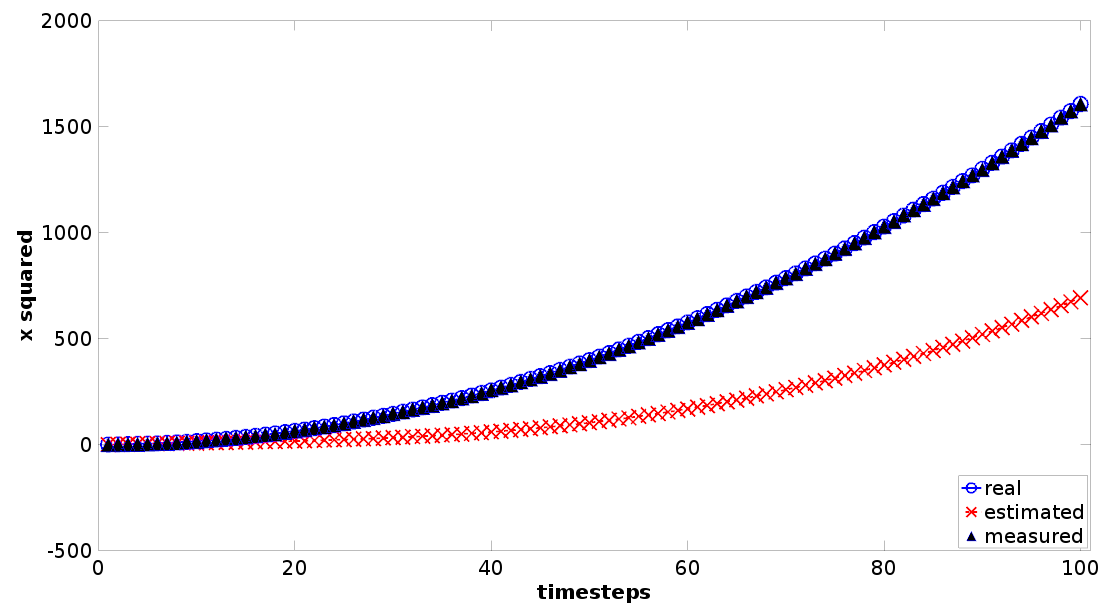
\includegraphics[width=\linewidth]{ox2_p001m1}
	\captionof{figure}{Stima di $x^2$ nelle prime 100 iterazioni, ponendo $\sigma_{proc} = 0.01$ e $\sigma_{meas} = 1$.} 
	\label{ox2_p001m1} 
\end{minipage}

\begin{minipage}{\linewidth}
	\centering
	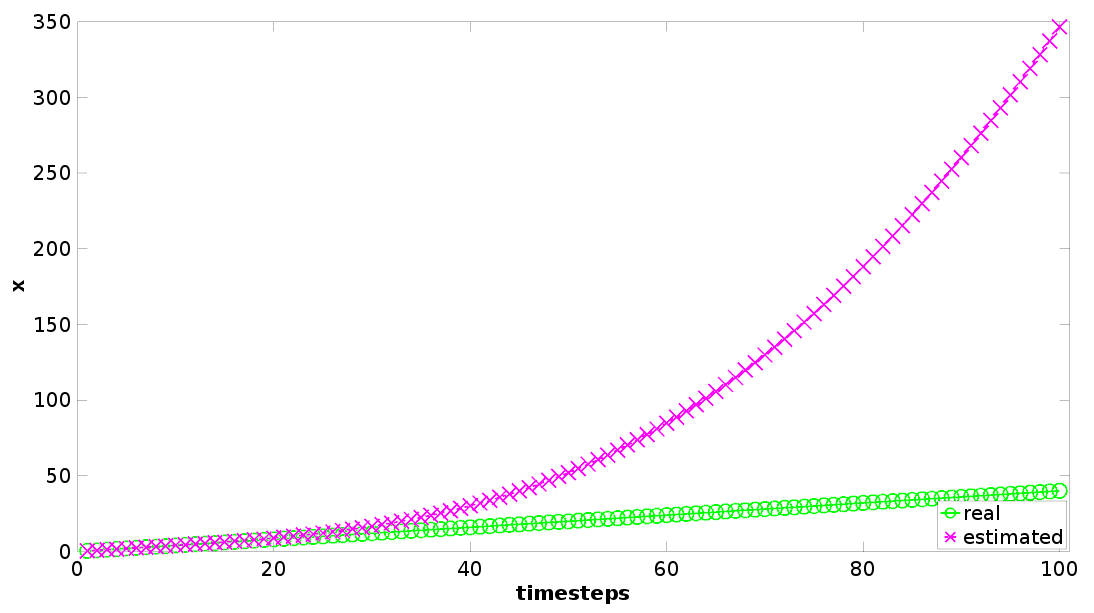
\includegraphics[width=\linewidth]{ox2_p001m1_x}
	\captionof{figure}{Stima di $x$ nelle prime 100 iterazioni, ponendo $\sigma_{proc} = 0.01$ e $\sigma_{meas} = 1$.} 
	\label{ox2_p001m1_x}
\end{minipage}

Al contrario, se il rumore di processo è alto rispetto al rumore di misurazione ($\sigma_{proc} = 1$ e $\sigma_{meas} = 0.01$), lo stimatore si affida alle osservazioni. In questo caso il Kalman filter approssima piuttosto bene il valore di $x^2$, ma il valore di $x$ risulta comunque estremamente inaccurato a causa del modello di transizione lineare: proprio quest'ultimo è infatti l'unico mezzo di cui il Kalman filter dispone per effettuare una stima di $x$.

\begin{minipage}{\linewidth}
	\centering
	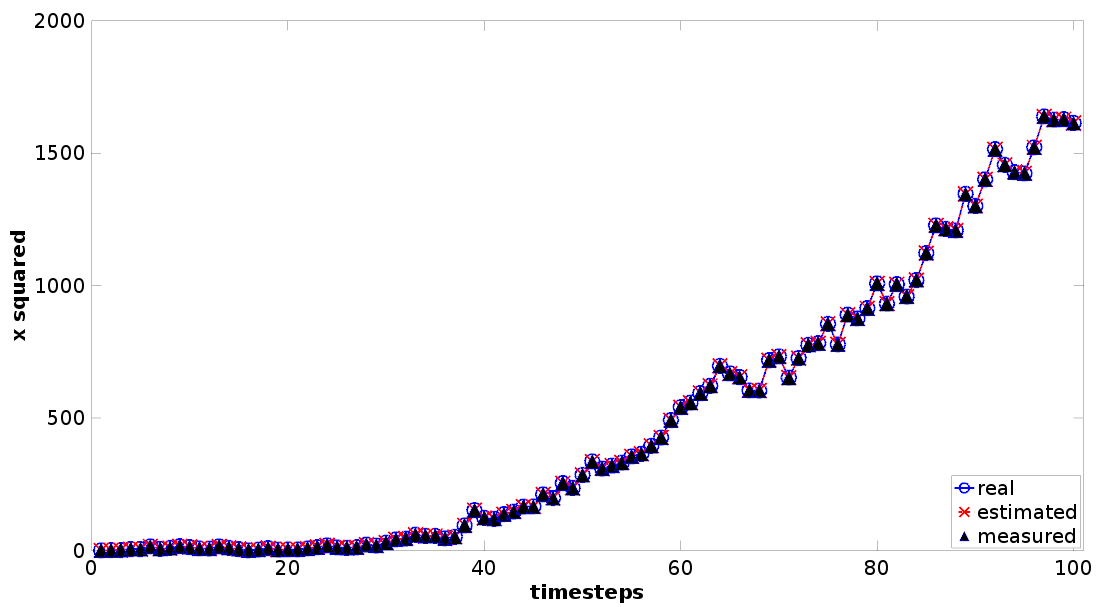
\includegraphics[width=\linewidth]{ox2_p1m001}
	\captionof{figure}{Stima di $x^2$ nelle prime 100 iterazioni, ponendo $\sigma_{proc} = 1$ e $\sigma_{meas} = 0.01$.} 
	\label{ps_a0m100} 
\end{minipage}

\begin{minipage}{\linewidth}
	\centering
	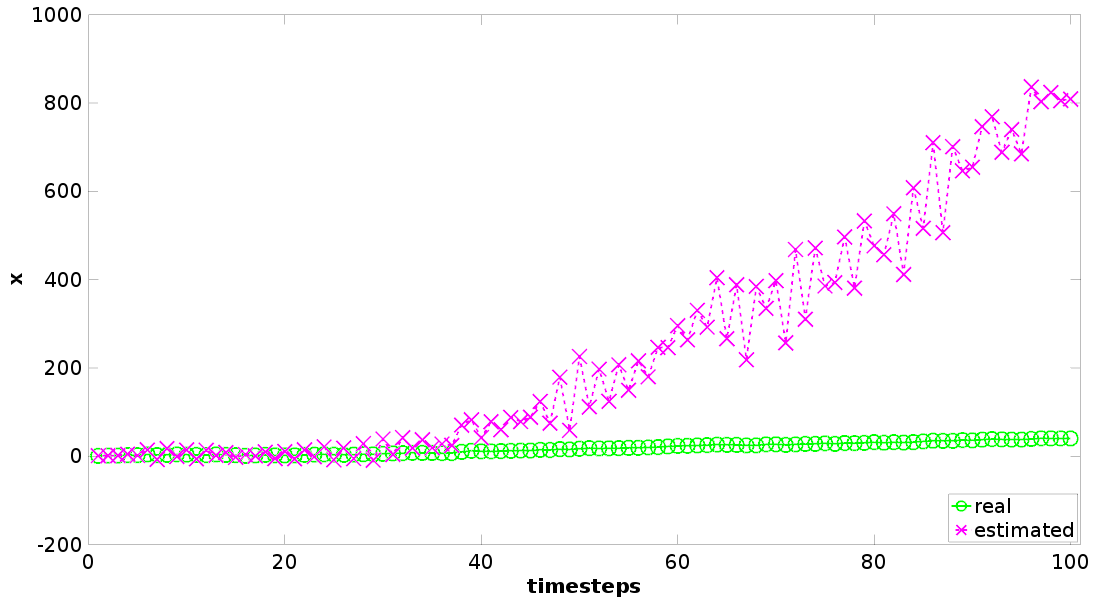
\includegraphics[width=\linewidth]{ox2_p1m001_x}
	\captionof{figure}{Stima di $x$ nelle prime 100 iterazioni, ponendo $\sigma_{proc} = 1$ e $\sigma_{meas} = 0.01$.} 
	\label{ws_a0m100_long}
\end{minipage}

\newpage

\item \textbf{Osservazione di $x$}\\
Se la variabile di stato osservata non è $x^2$ bensì $x$, la situazione generale non migliora: il Kalman filter, potenzialmente, riesce ad approssimare bene $x$; nonostante ciò l'errore commesso nella stima di $x^2$ è destinato ad aumentare man mano che ci si allontana dal punto in cui è stata calcolata la formula di Taylor (dove l'approssimazione lineare della funzione quadratica risulta ottimale). 
\end{itemize}

In conclusione, il processo reale non può essere approssimato nella sua interezza a causa delle forti restrizioni imposte dal modello di transizione lineare. I risultati ottenuti suggeriscono tuttavia un possibile approccio per trattare anche processi non lineari: se si potesse calcolare ``dinamicamente" la formula di Taylor modificando il punto $a$ ad ogni iterazione, la simulazione del processo sarebbe decisamente migliore. Questa è l'idea che sta alla base del cosiddetto Extended Kalman Filter.











